\part{圆幂与根心}
% 相交弦定理





\section{圆幂}
% 圆幂定理
\begin{theorem}[圆幂定理]
    假设平面内有一半径为R的圆O,P为平面内任意一点。
    
    从P作圆O的任一割线PAB,从点P起到与圆周相交为止的两线段之积$PA\cdot PB$,称作点P到圆O的圆幂。
    
    P到圆O的圆幂等于$|OP^2 - R^2|$。
\end{theorem}
\begin{figure}[H]
    \centering
    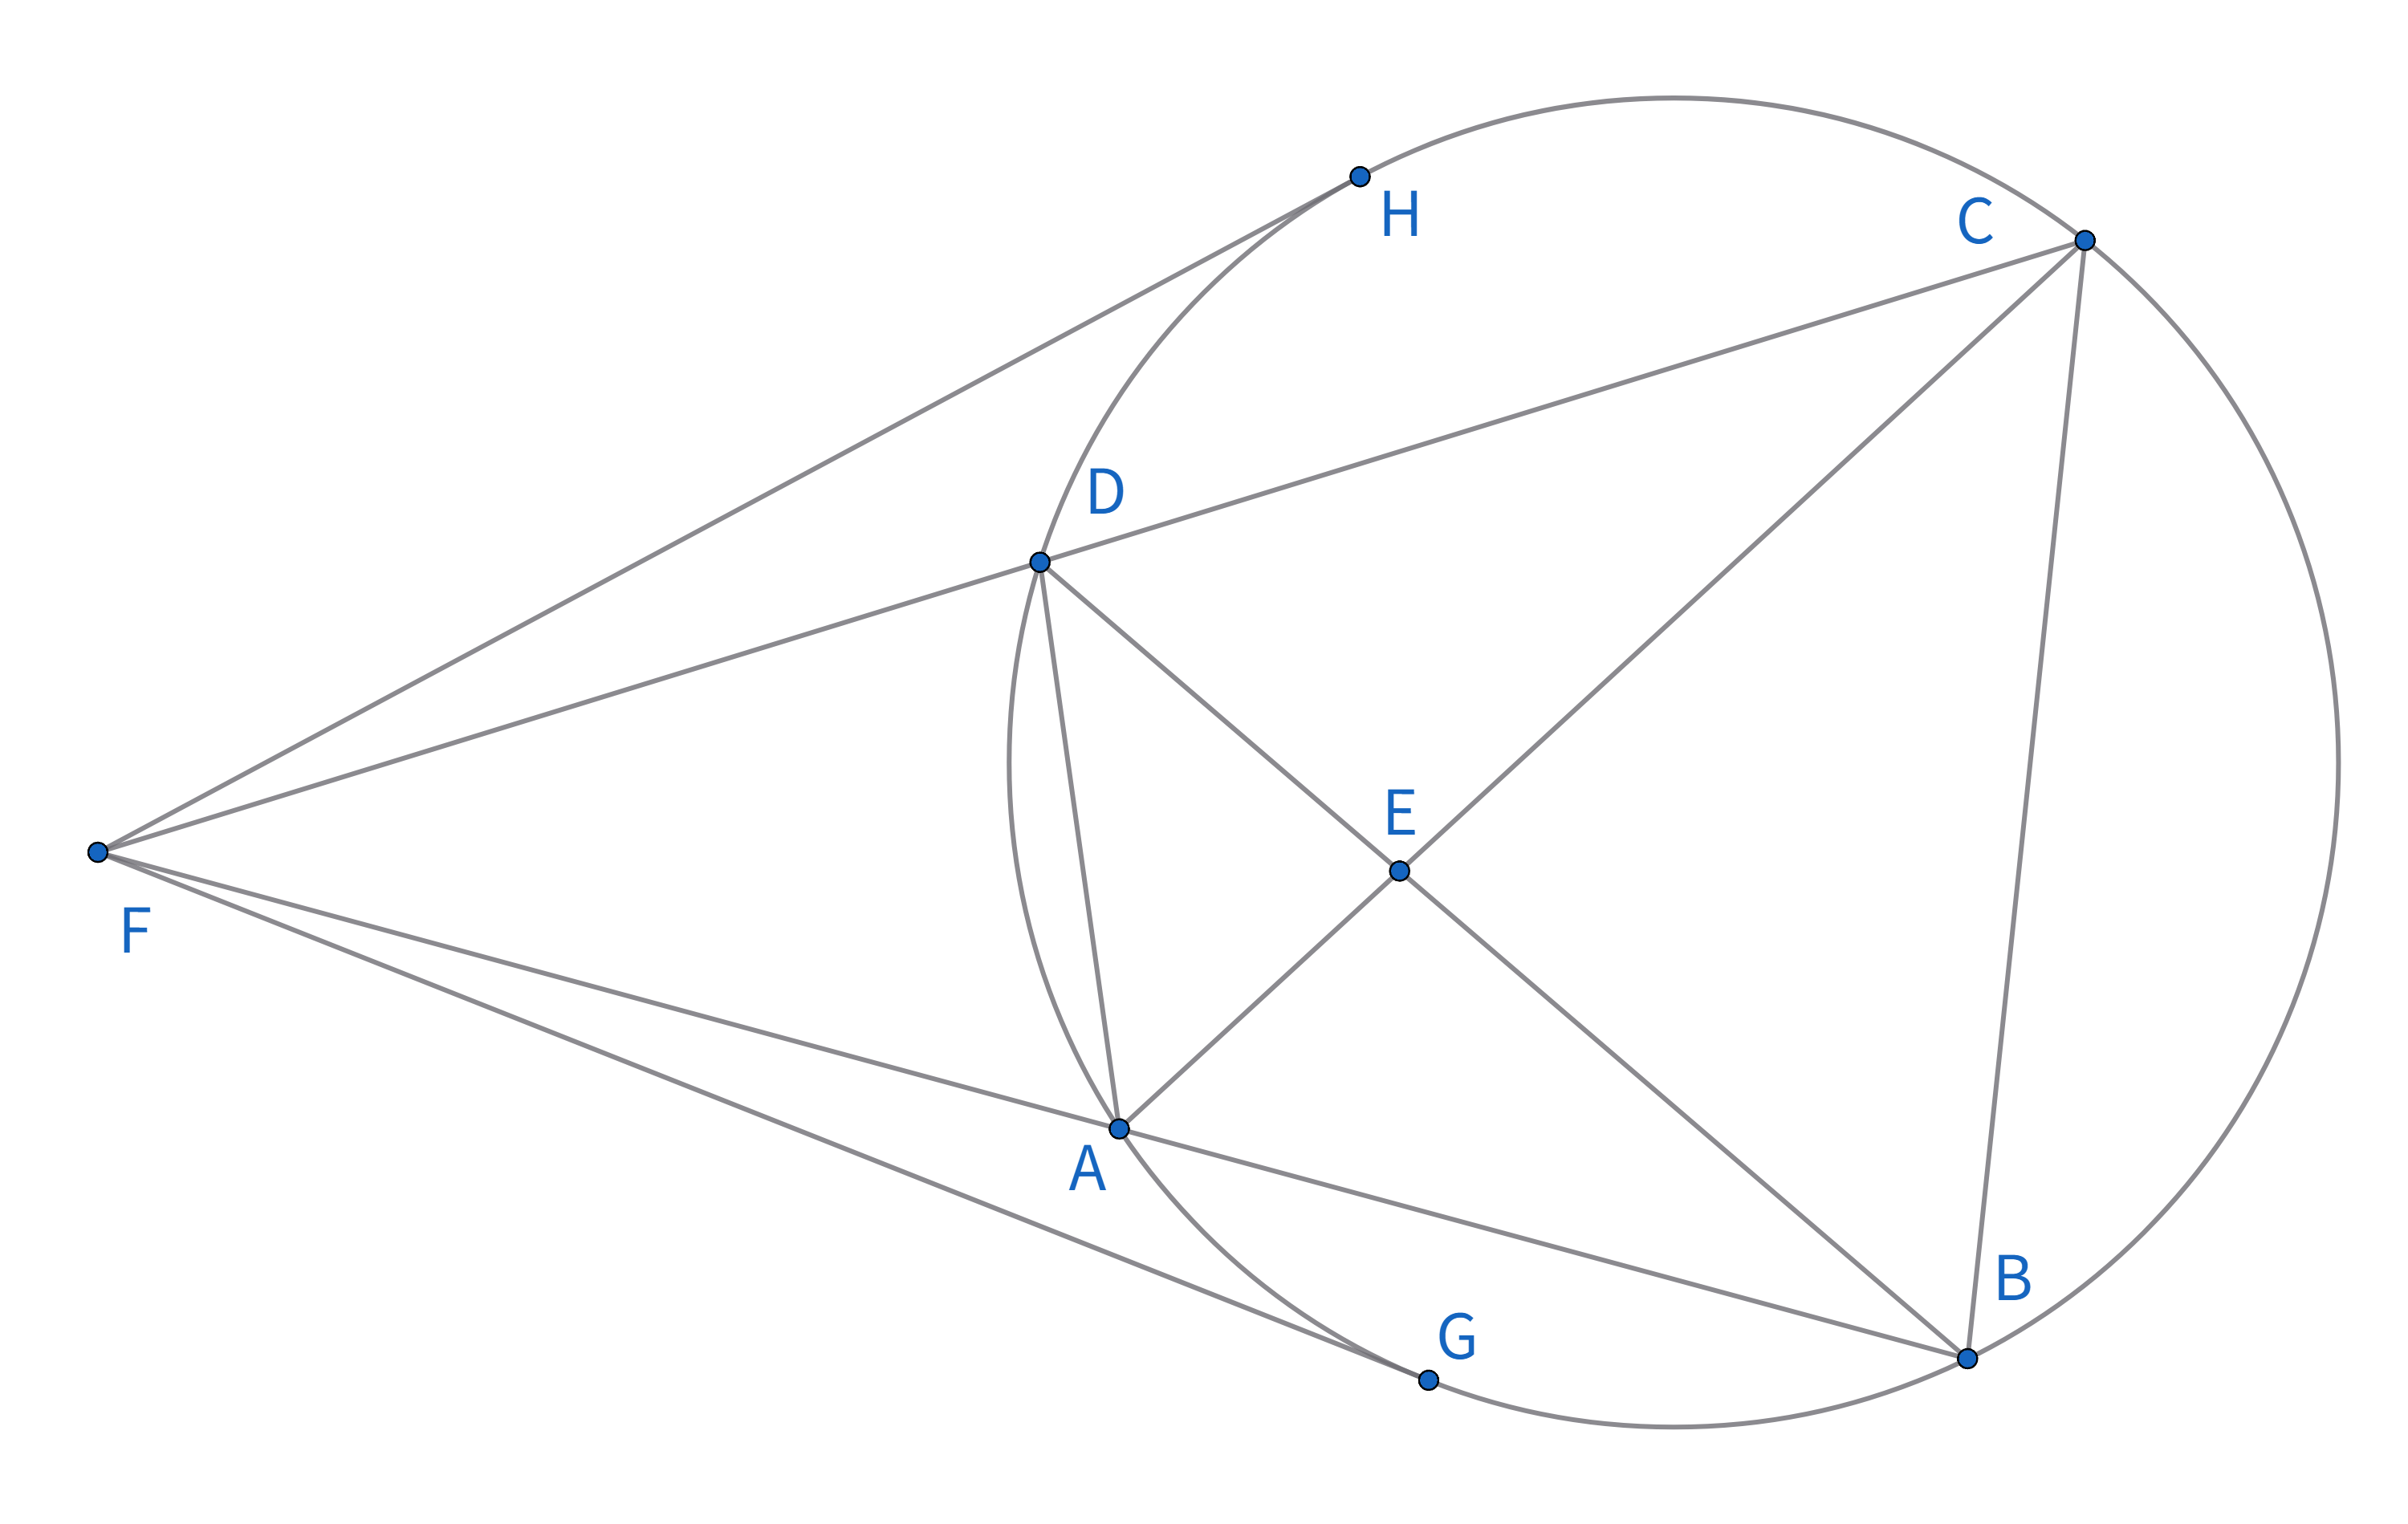
\includegraphics[width=0.7\linewidth]{figures/圆幂定理.png}
    \caption{圆幂定理}
\end{figure}
\begin{remark}
    定点到定圆的圆幂是一个定值,与割线的取法无关。
\end{remark}

%-------------------------------------------------------------
\newpage 
\subsection{根轴}
\begin{theorem}[根轴]
    对于两已知圆有等幂点的轨迹,为一条垂直于连心线的直线。
\end{theorem}
\begin{figure}[H]
    \centering
    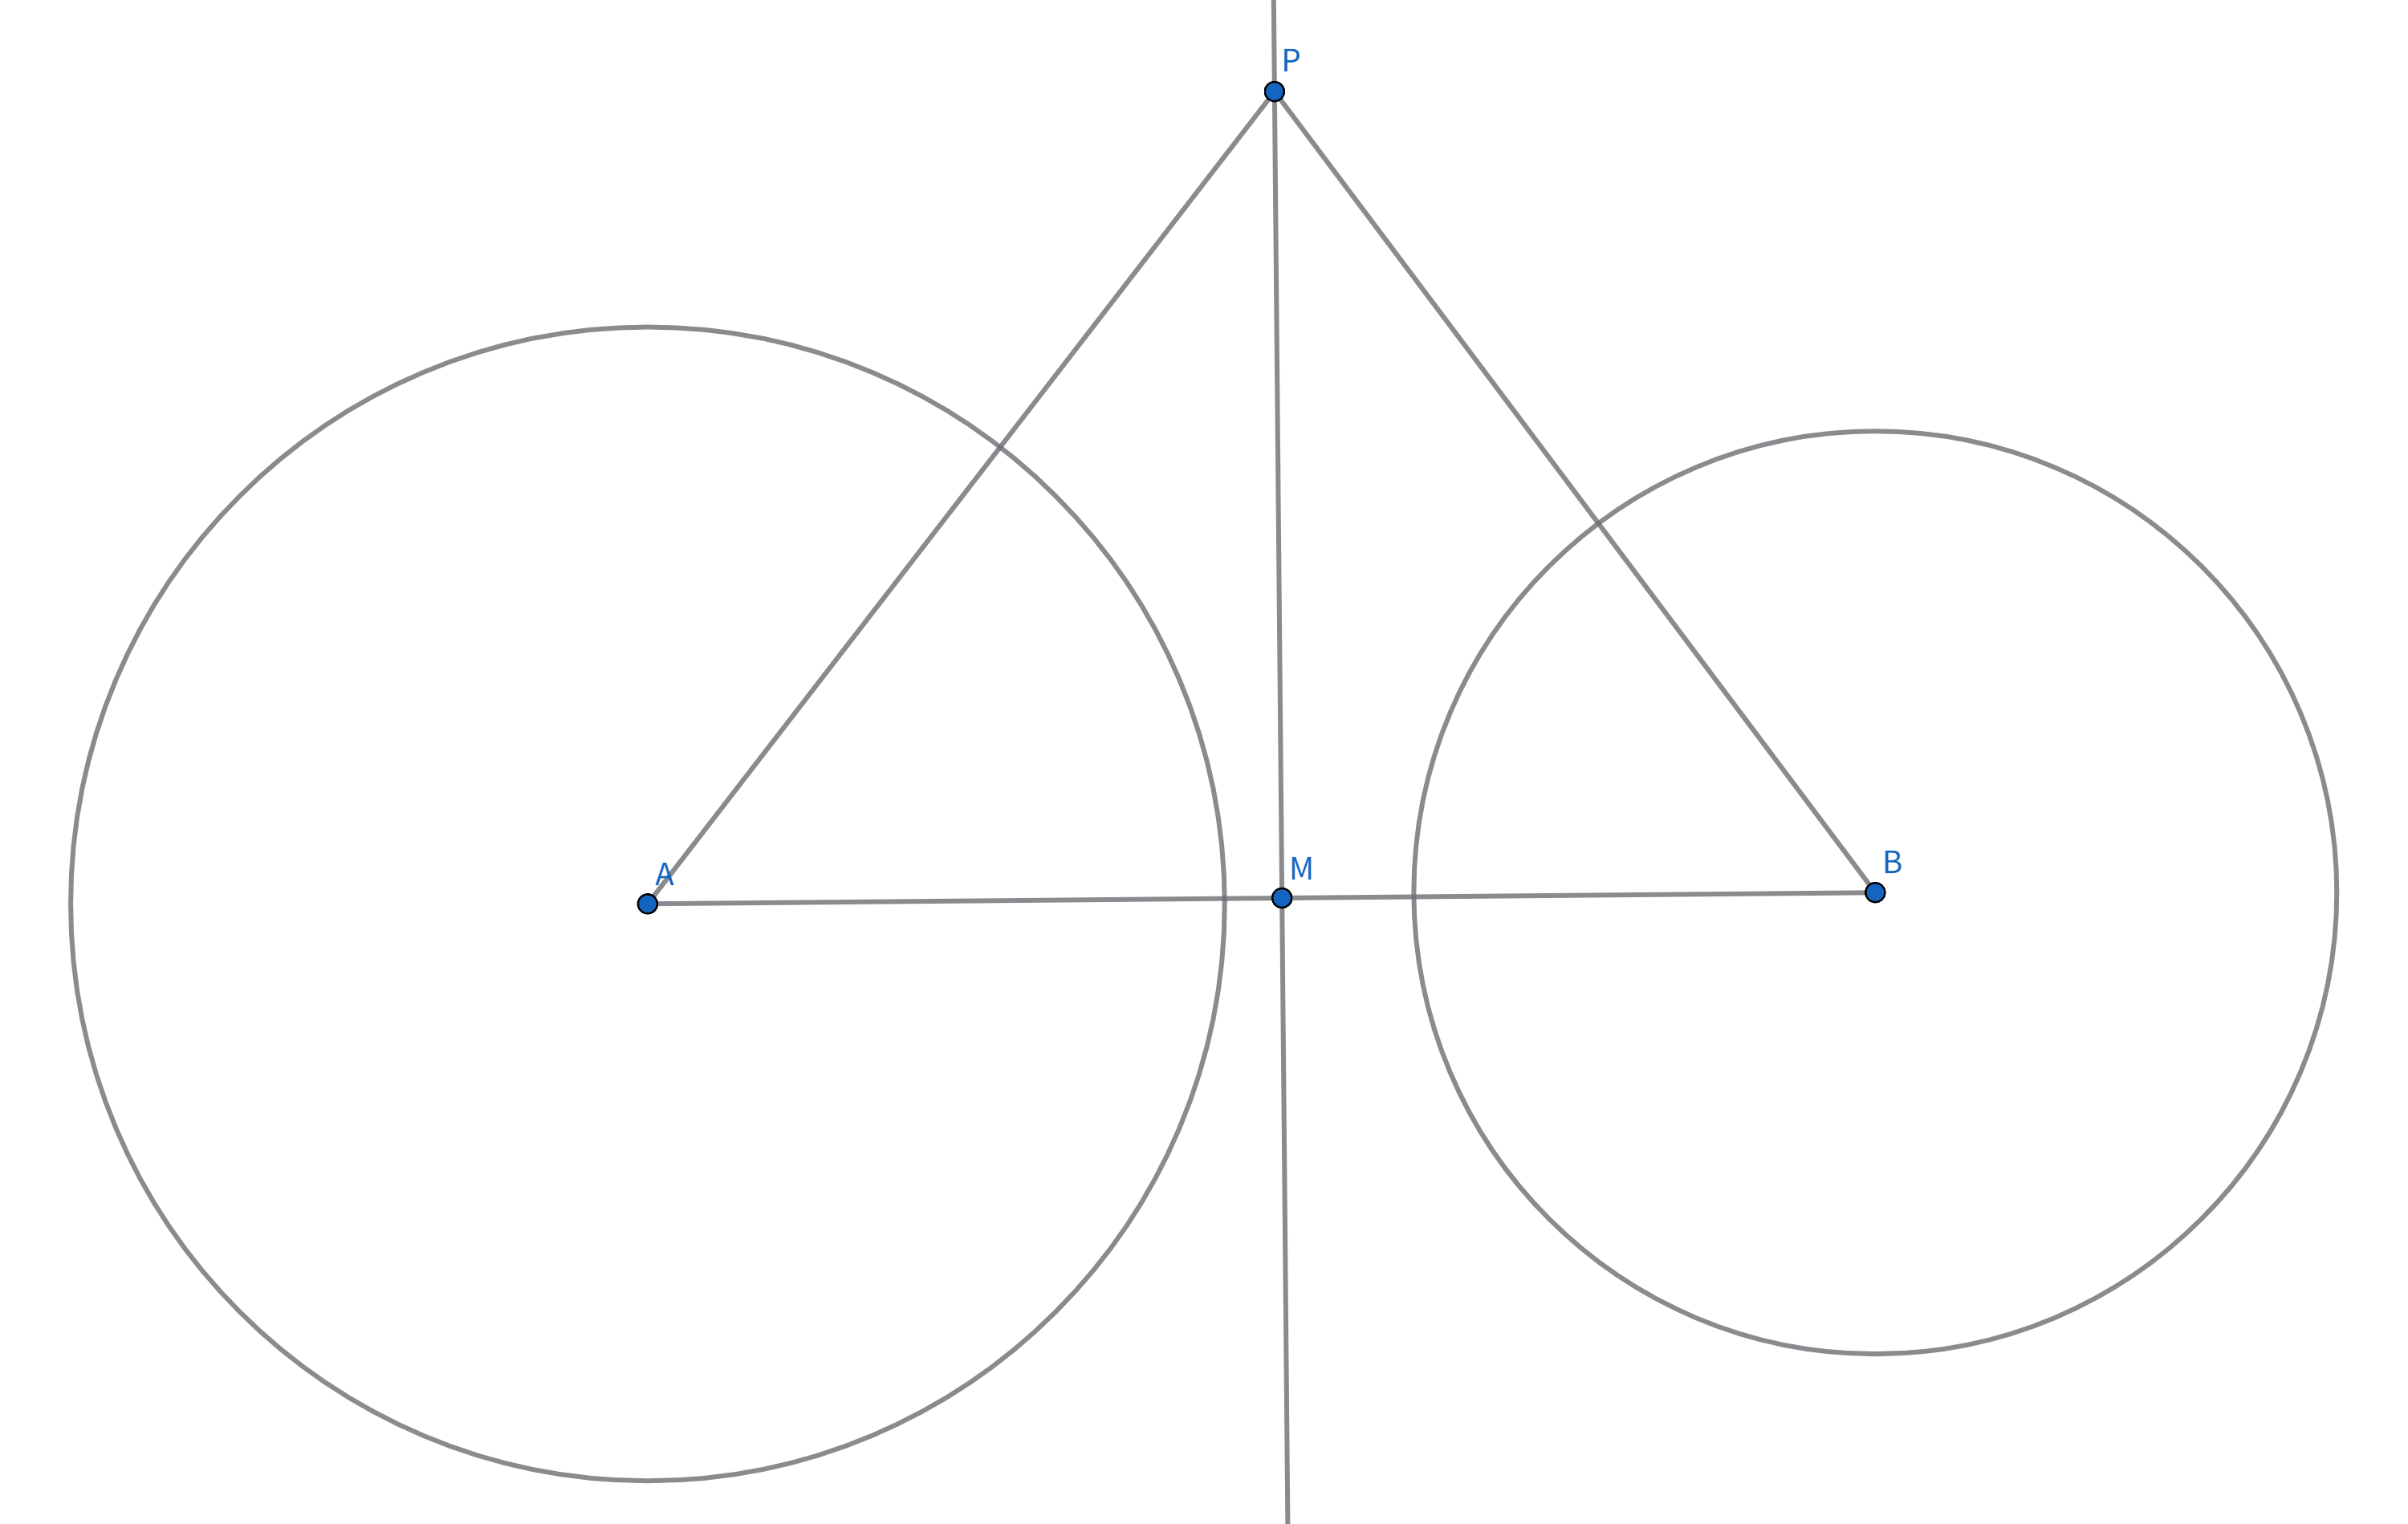
\includegraphics[width=0.7\linewidth]{figures/根轴.png}
    \caption{根轴}
\end{figure}

\begin{proposition}[根轴性质]
    两圆的根轴有如下性质:
    
    (1) 若两圆相交,其根轴就是公共弦所在的直线。
    
    (2) 若两圆相切(内切或外切),其根轴就是过两圆切点的公切线。
    
    (3) 若两圆外离,则两圆的四条公切线的中点在根轴上。
\end{proposition}
\begin{figure}[H]
    \centering
    \hfill % 添加一些水平间距
    \begin{minipage}[t]{0.3\textwidth}
        \centering
        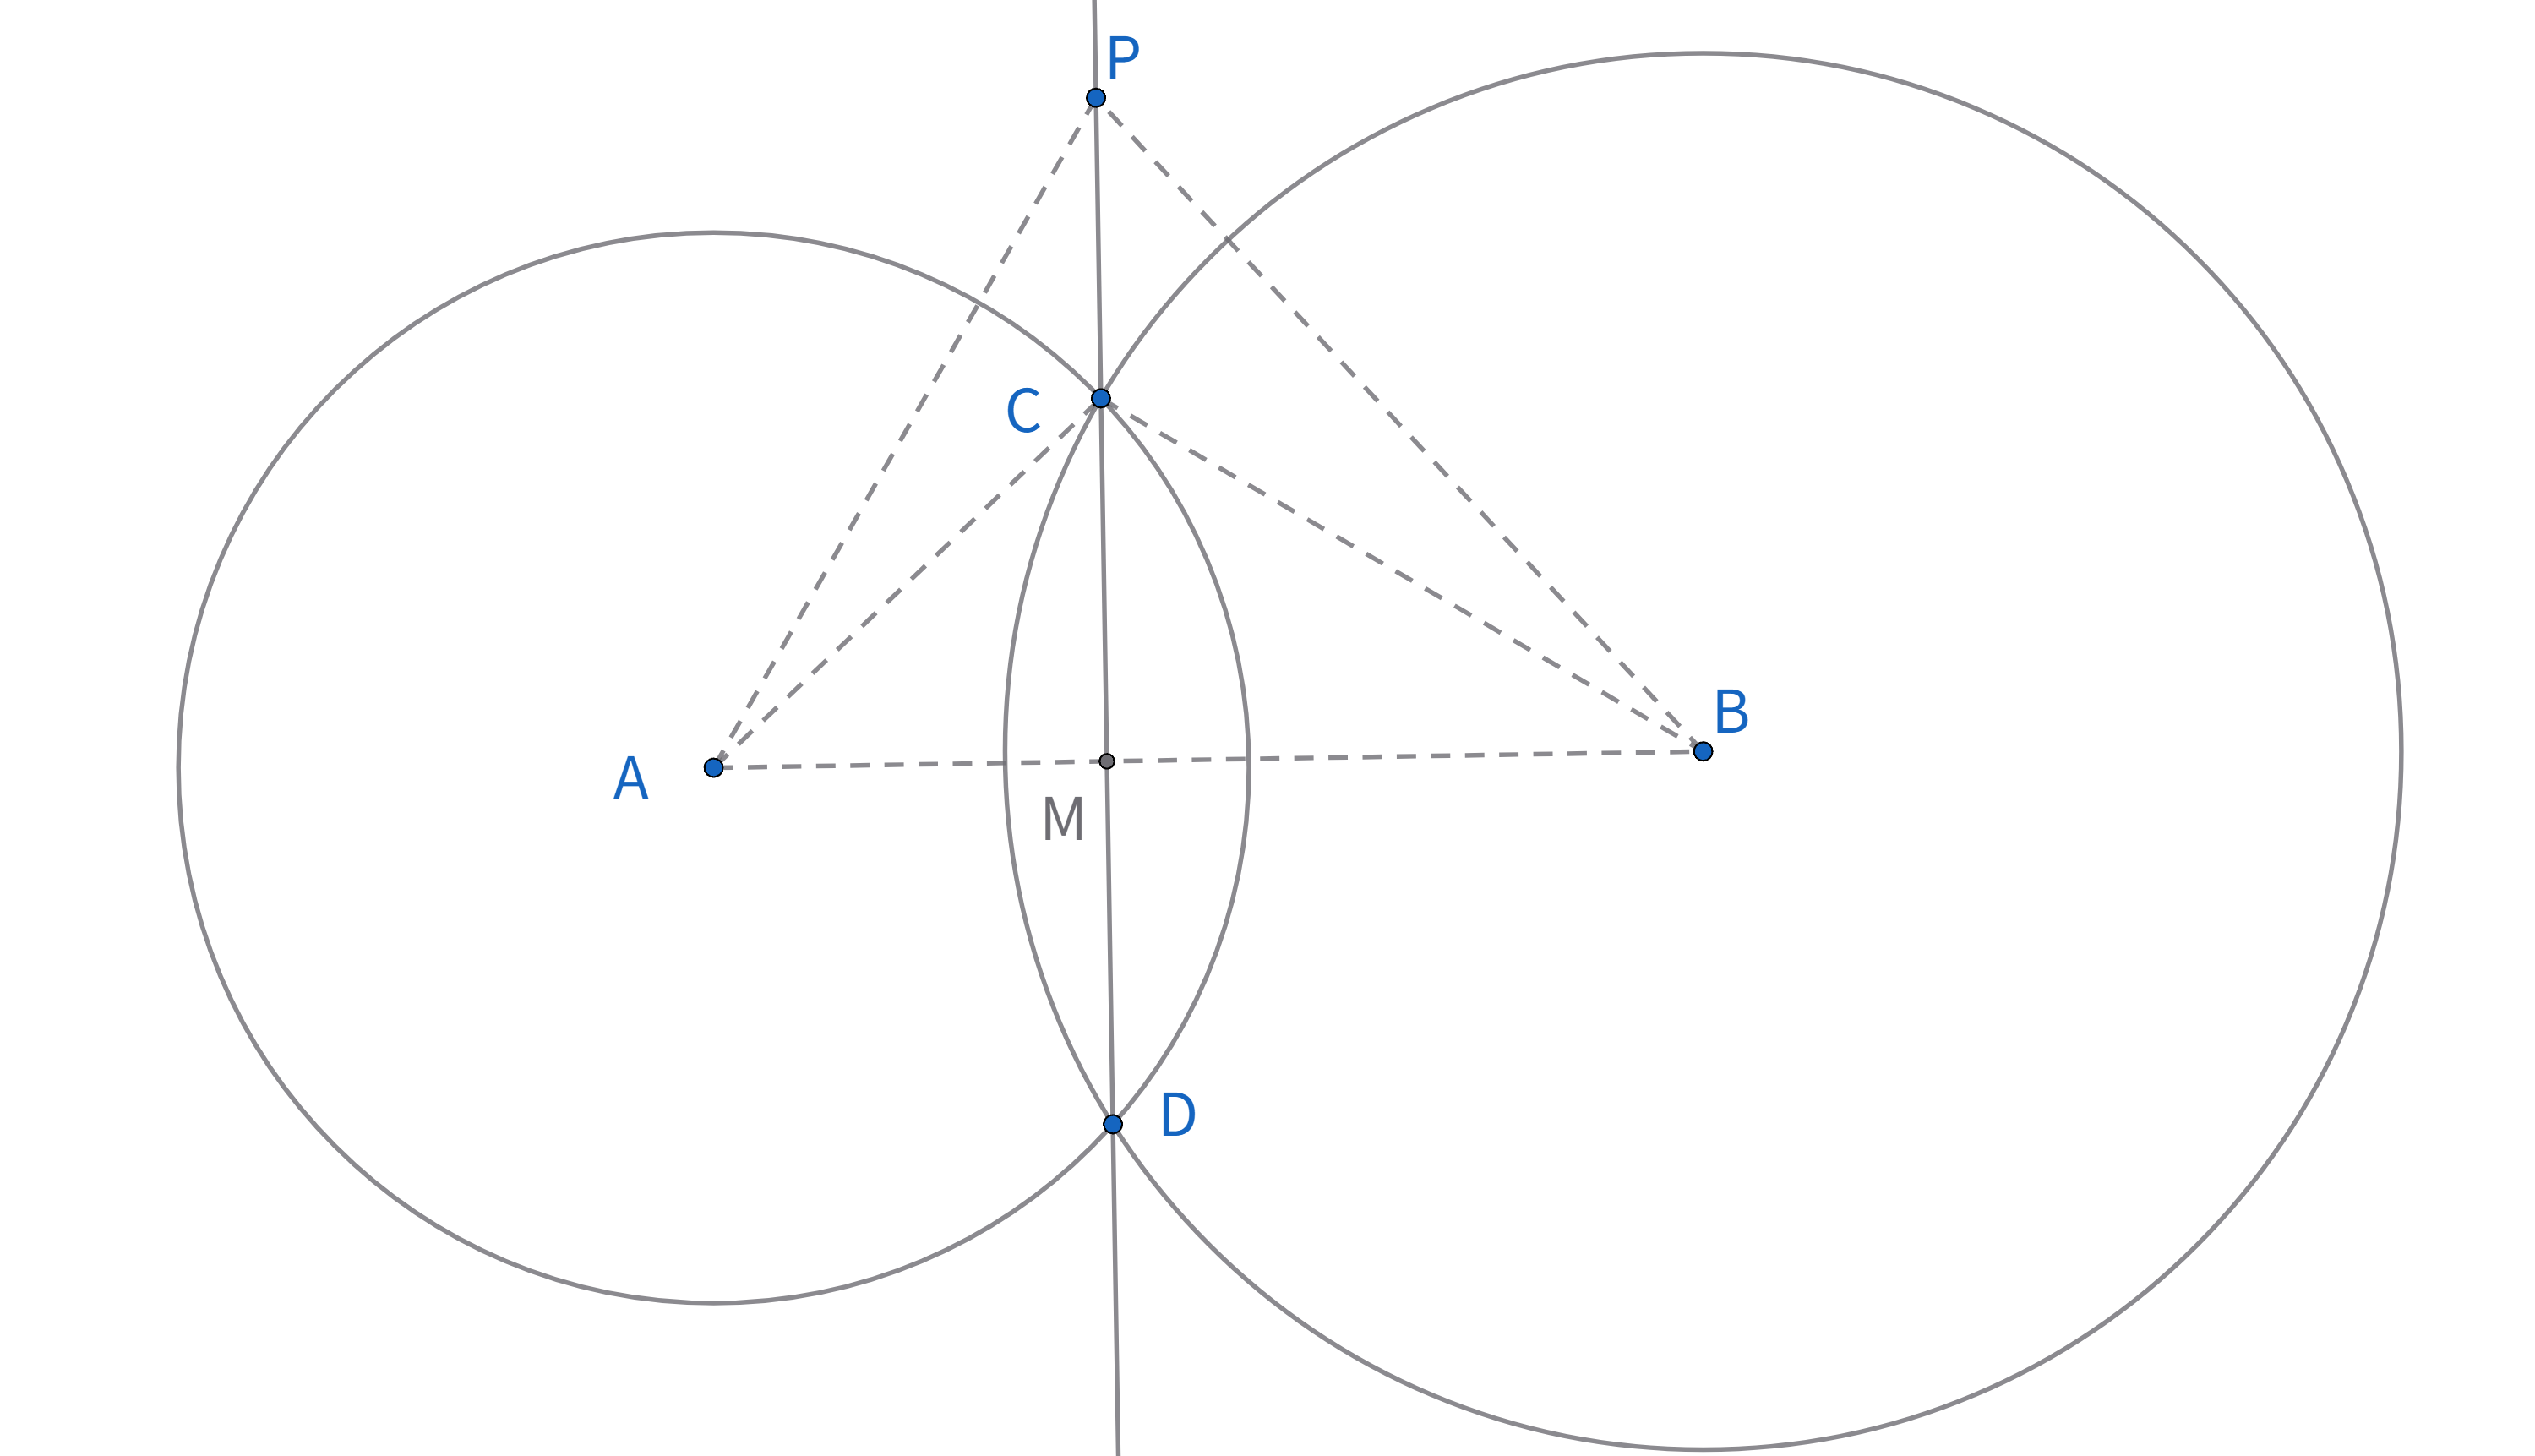
\includegraphics[width=\linewidth]{figures/相交圆根轴.png}
        \caption{相交圆根轴}
    \end{minipage}
    \hfill % 添加一些水平间距
    \begin{minipage}[t]{0.3\textwidth}
    \centering
    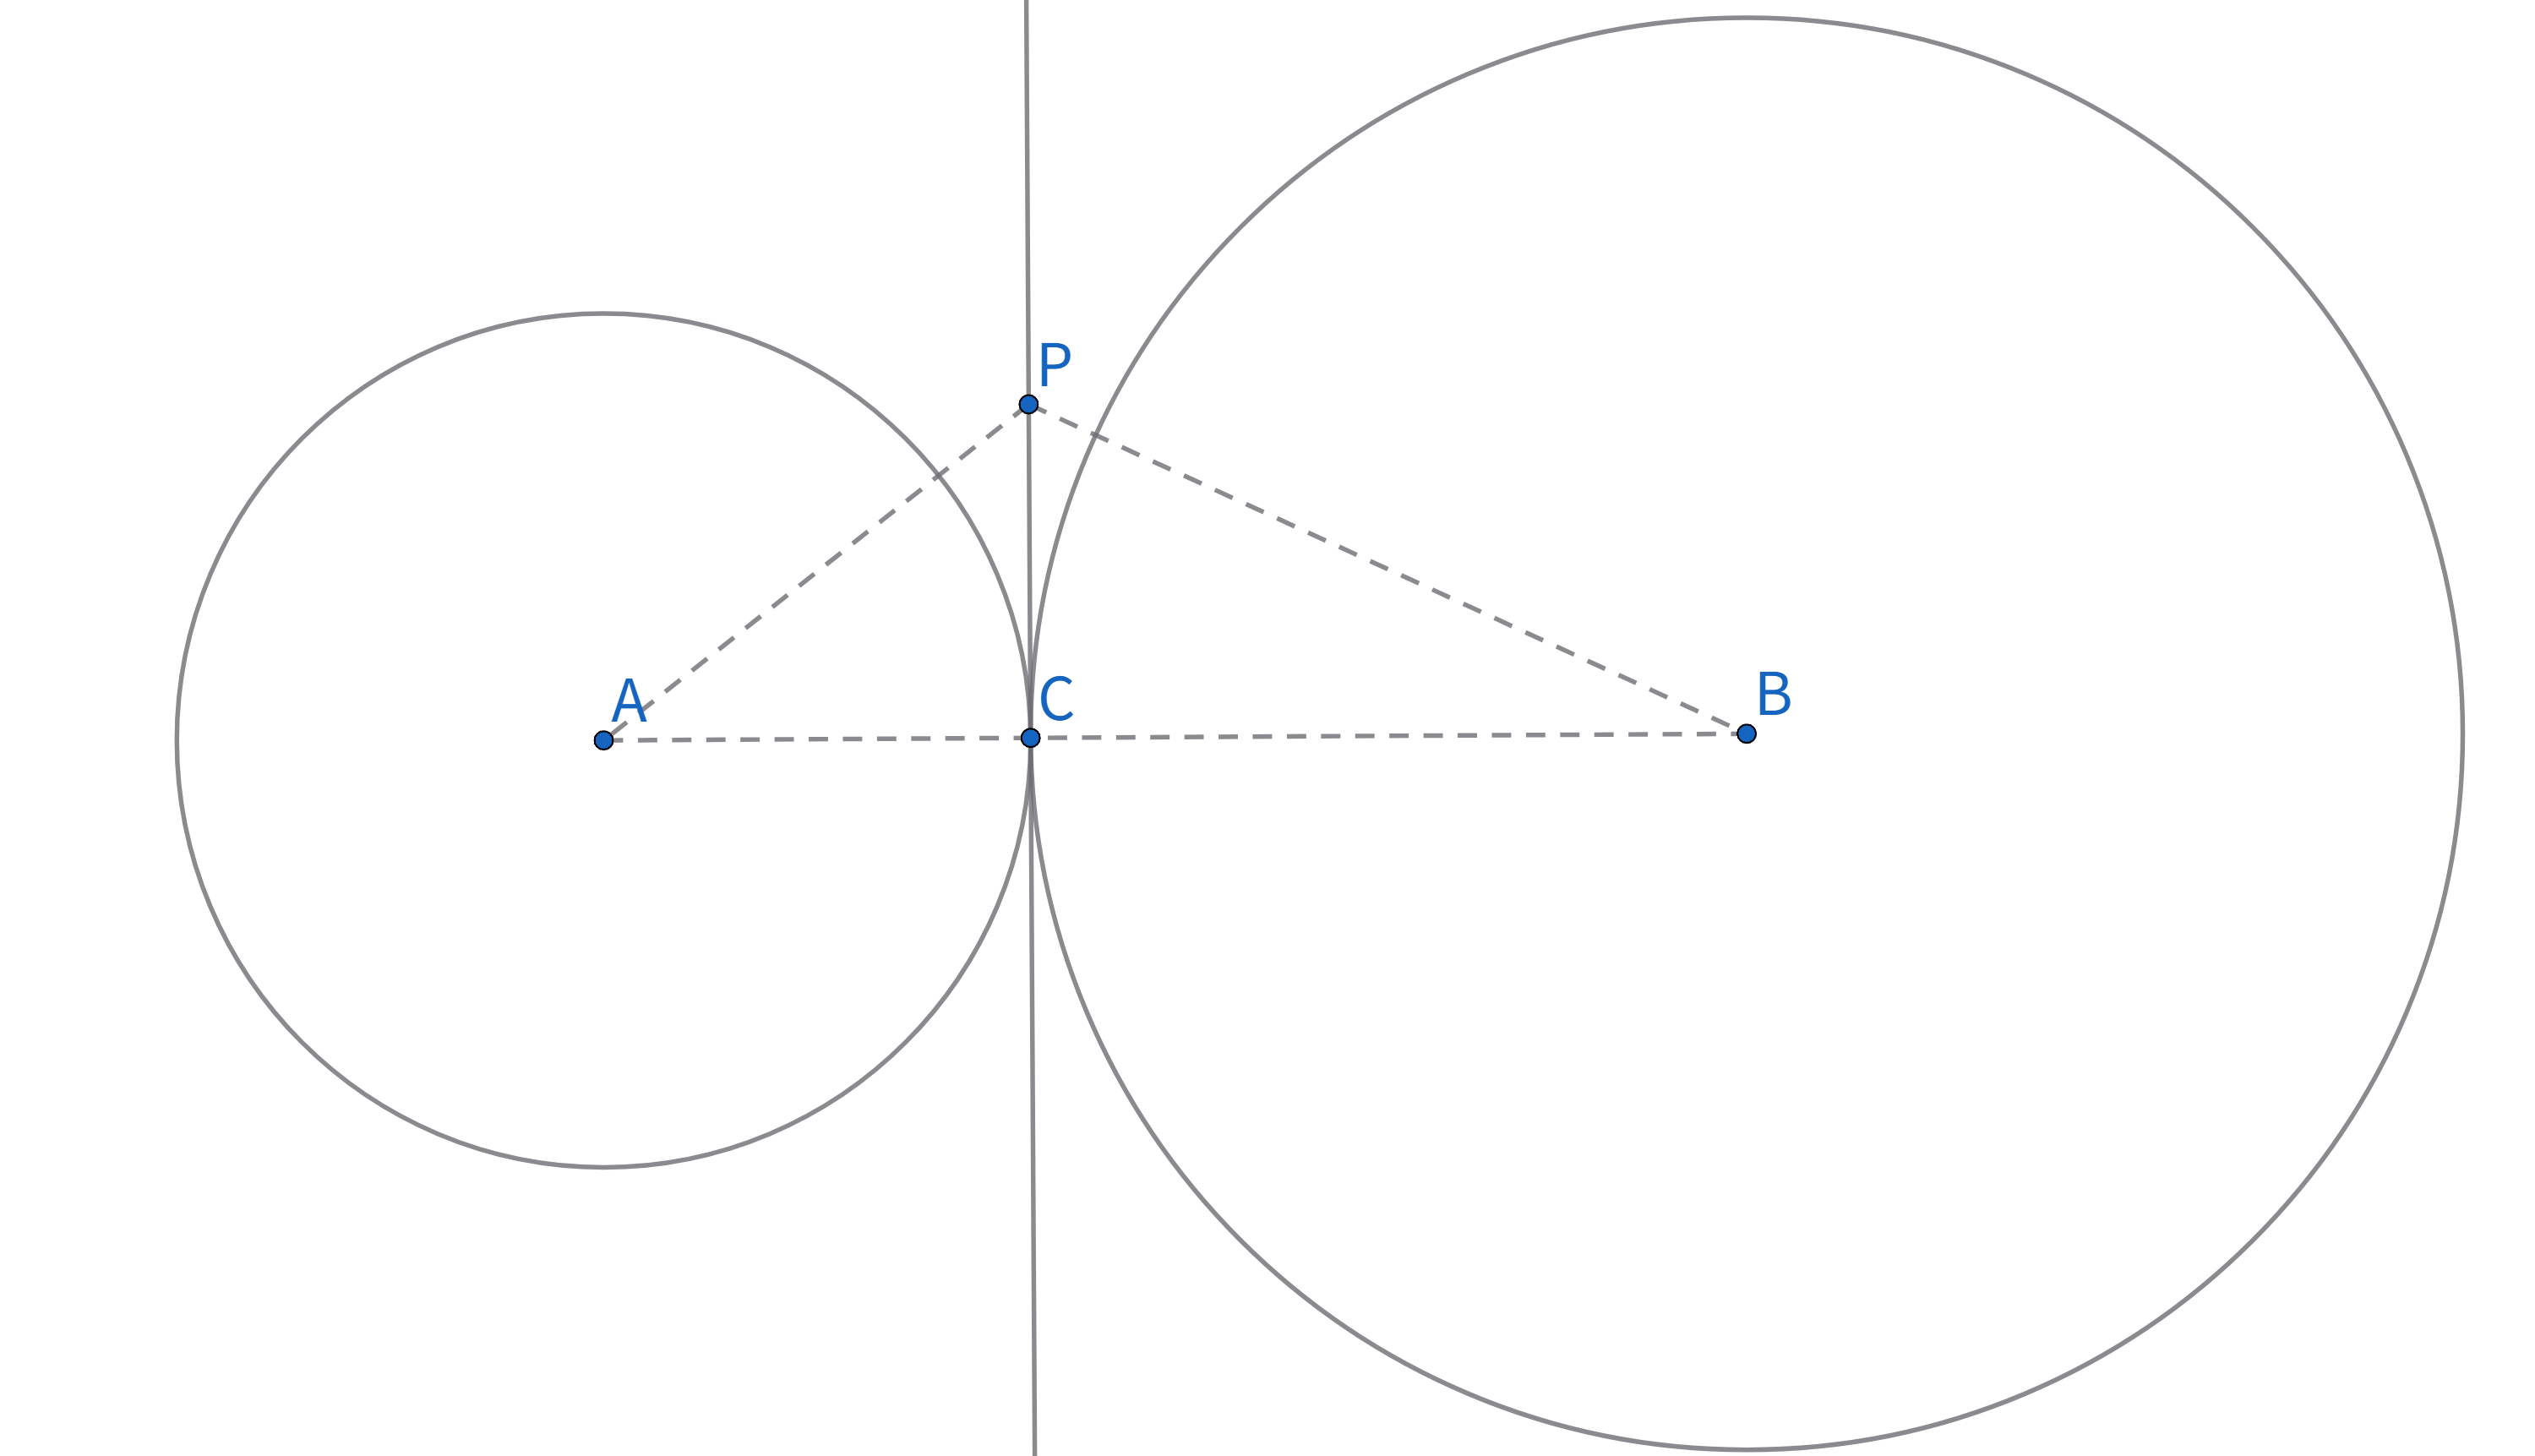
\includegraphics[width=\linewidth]{figures/相切圆根轴.png}
    \caption{相切圆根轴}
    \end{minipage}
    \begin{minipage}[t]{0.3\textwidth}
    \centering
    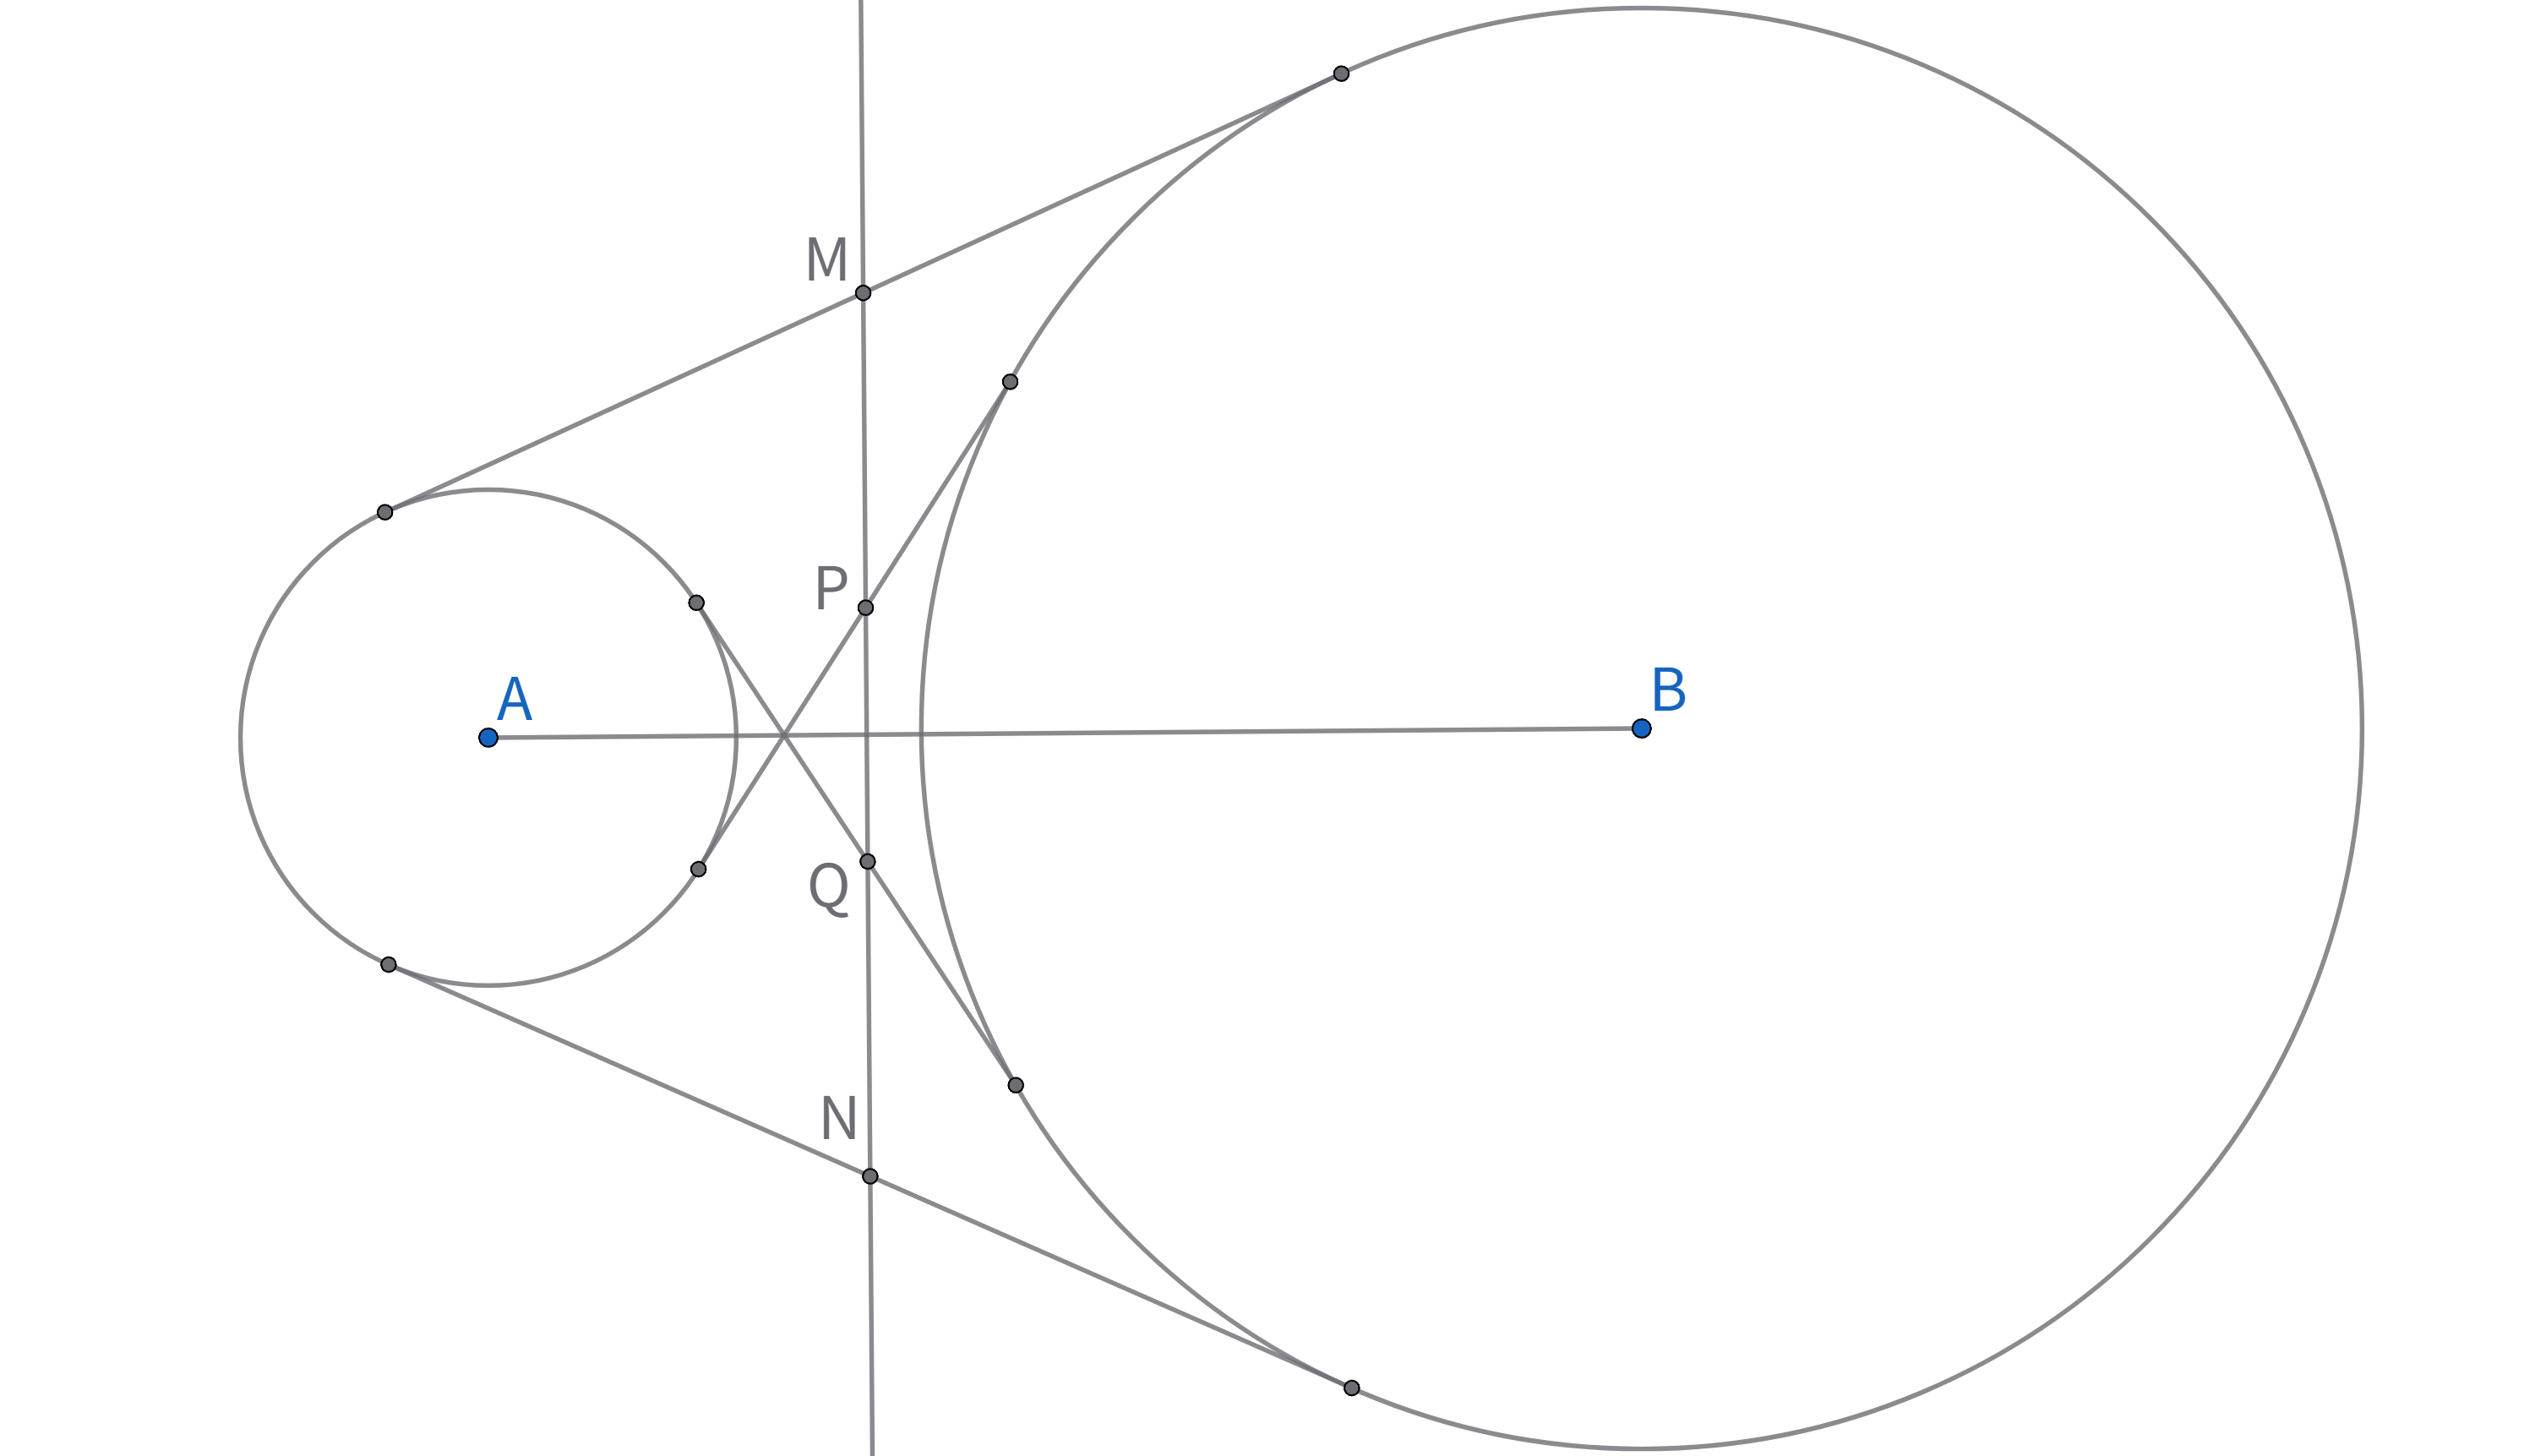
\includegraphics[width=\linewidth]{figures/相离圆根轴.png}
    \caption{相离圆根轴}
    \end{minipage}
\end{figure}


%-------------------------------------------------------------
\newpage 
\subsection{根心}
\begin{theorem}[根心定理]
    平面内的三个定圆,他们两两的根轴或相交于一点,或互相平行。
\end{theorem}
\begin{figure}[H]
    \centering
    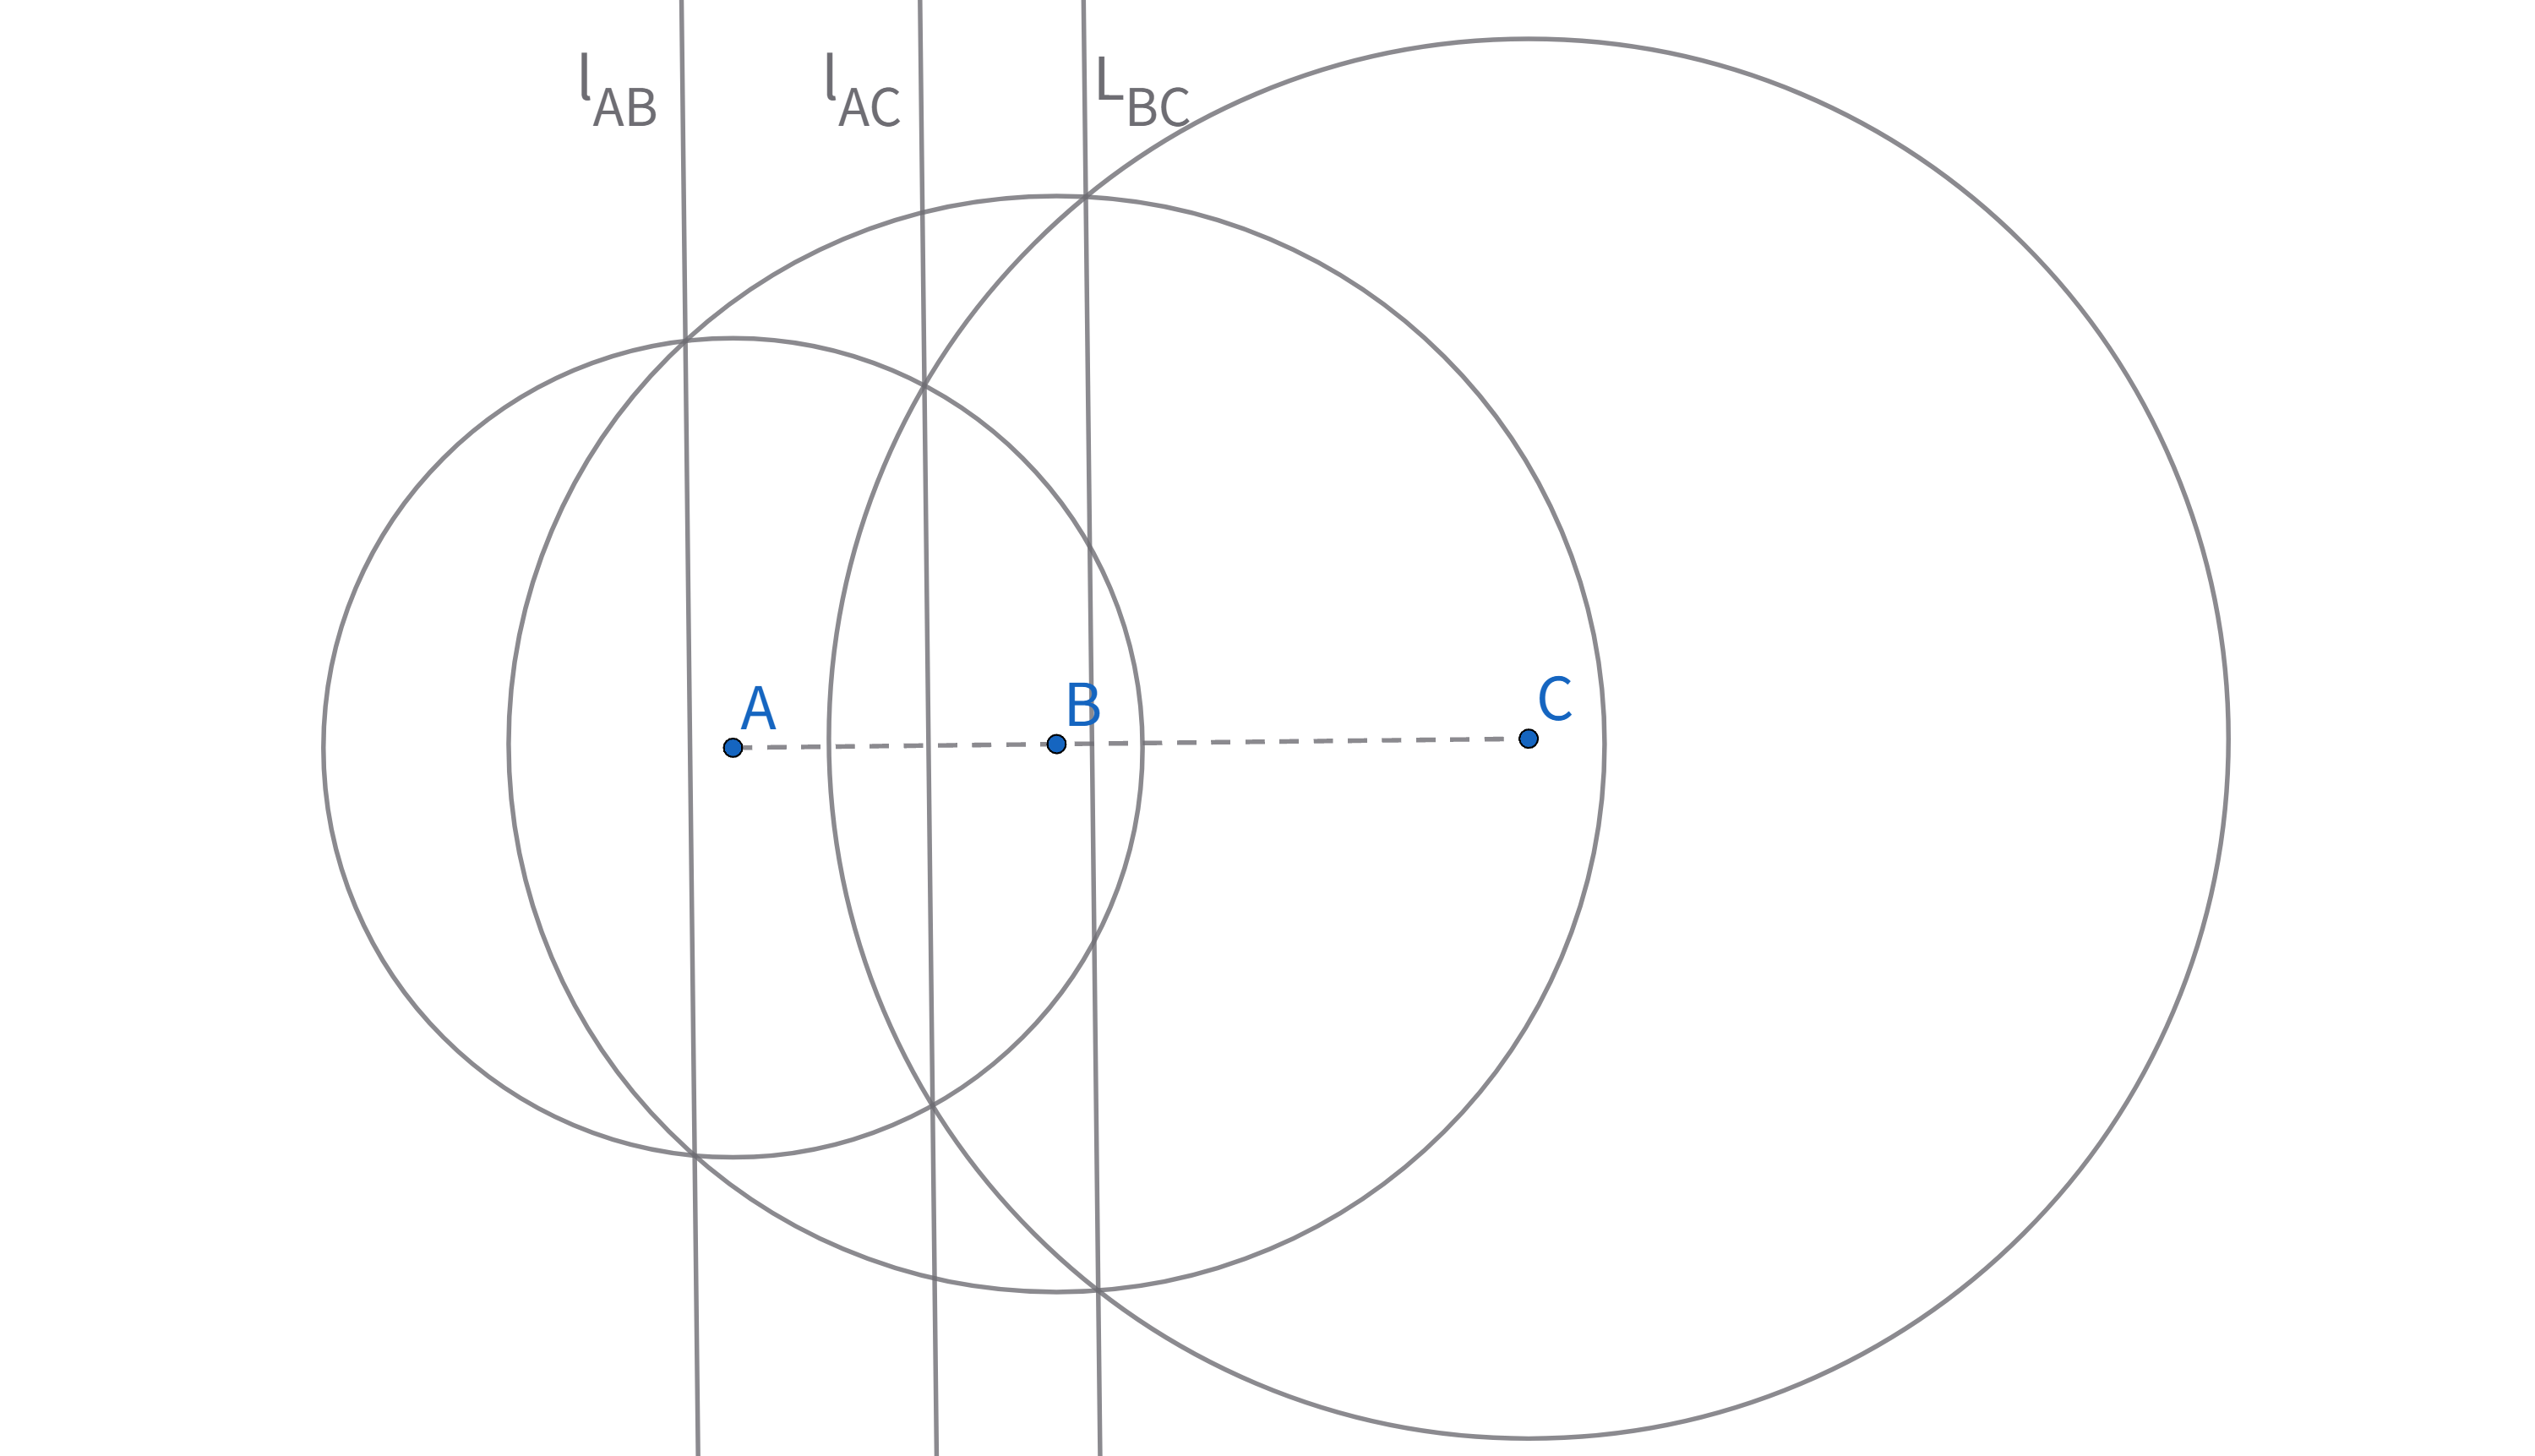
\includegraphics[width=0.8\linewidth]{figures/平行根轴.png}
    \caption{平行根轴}
\end{figure}
\begin{figure}[H]
    \centering
    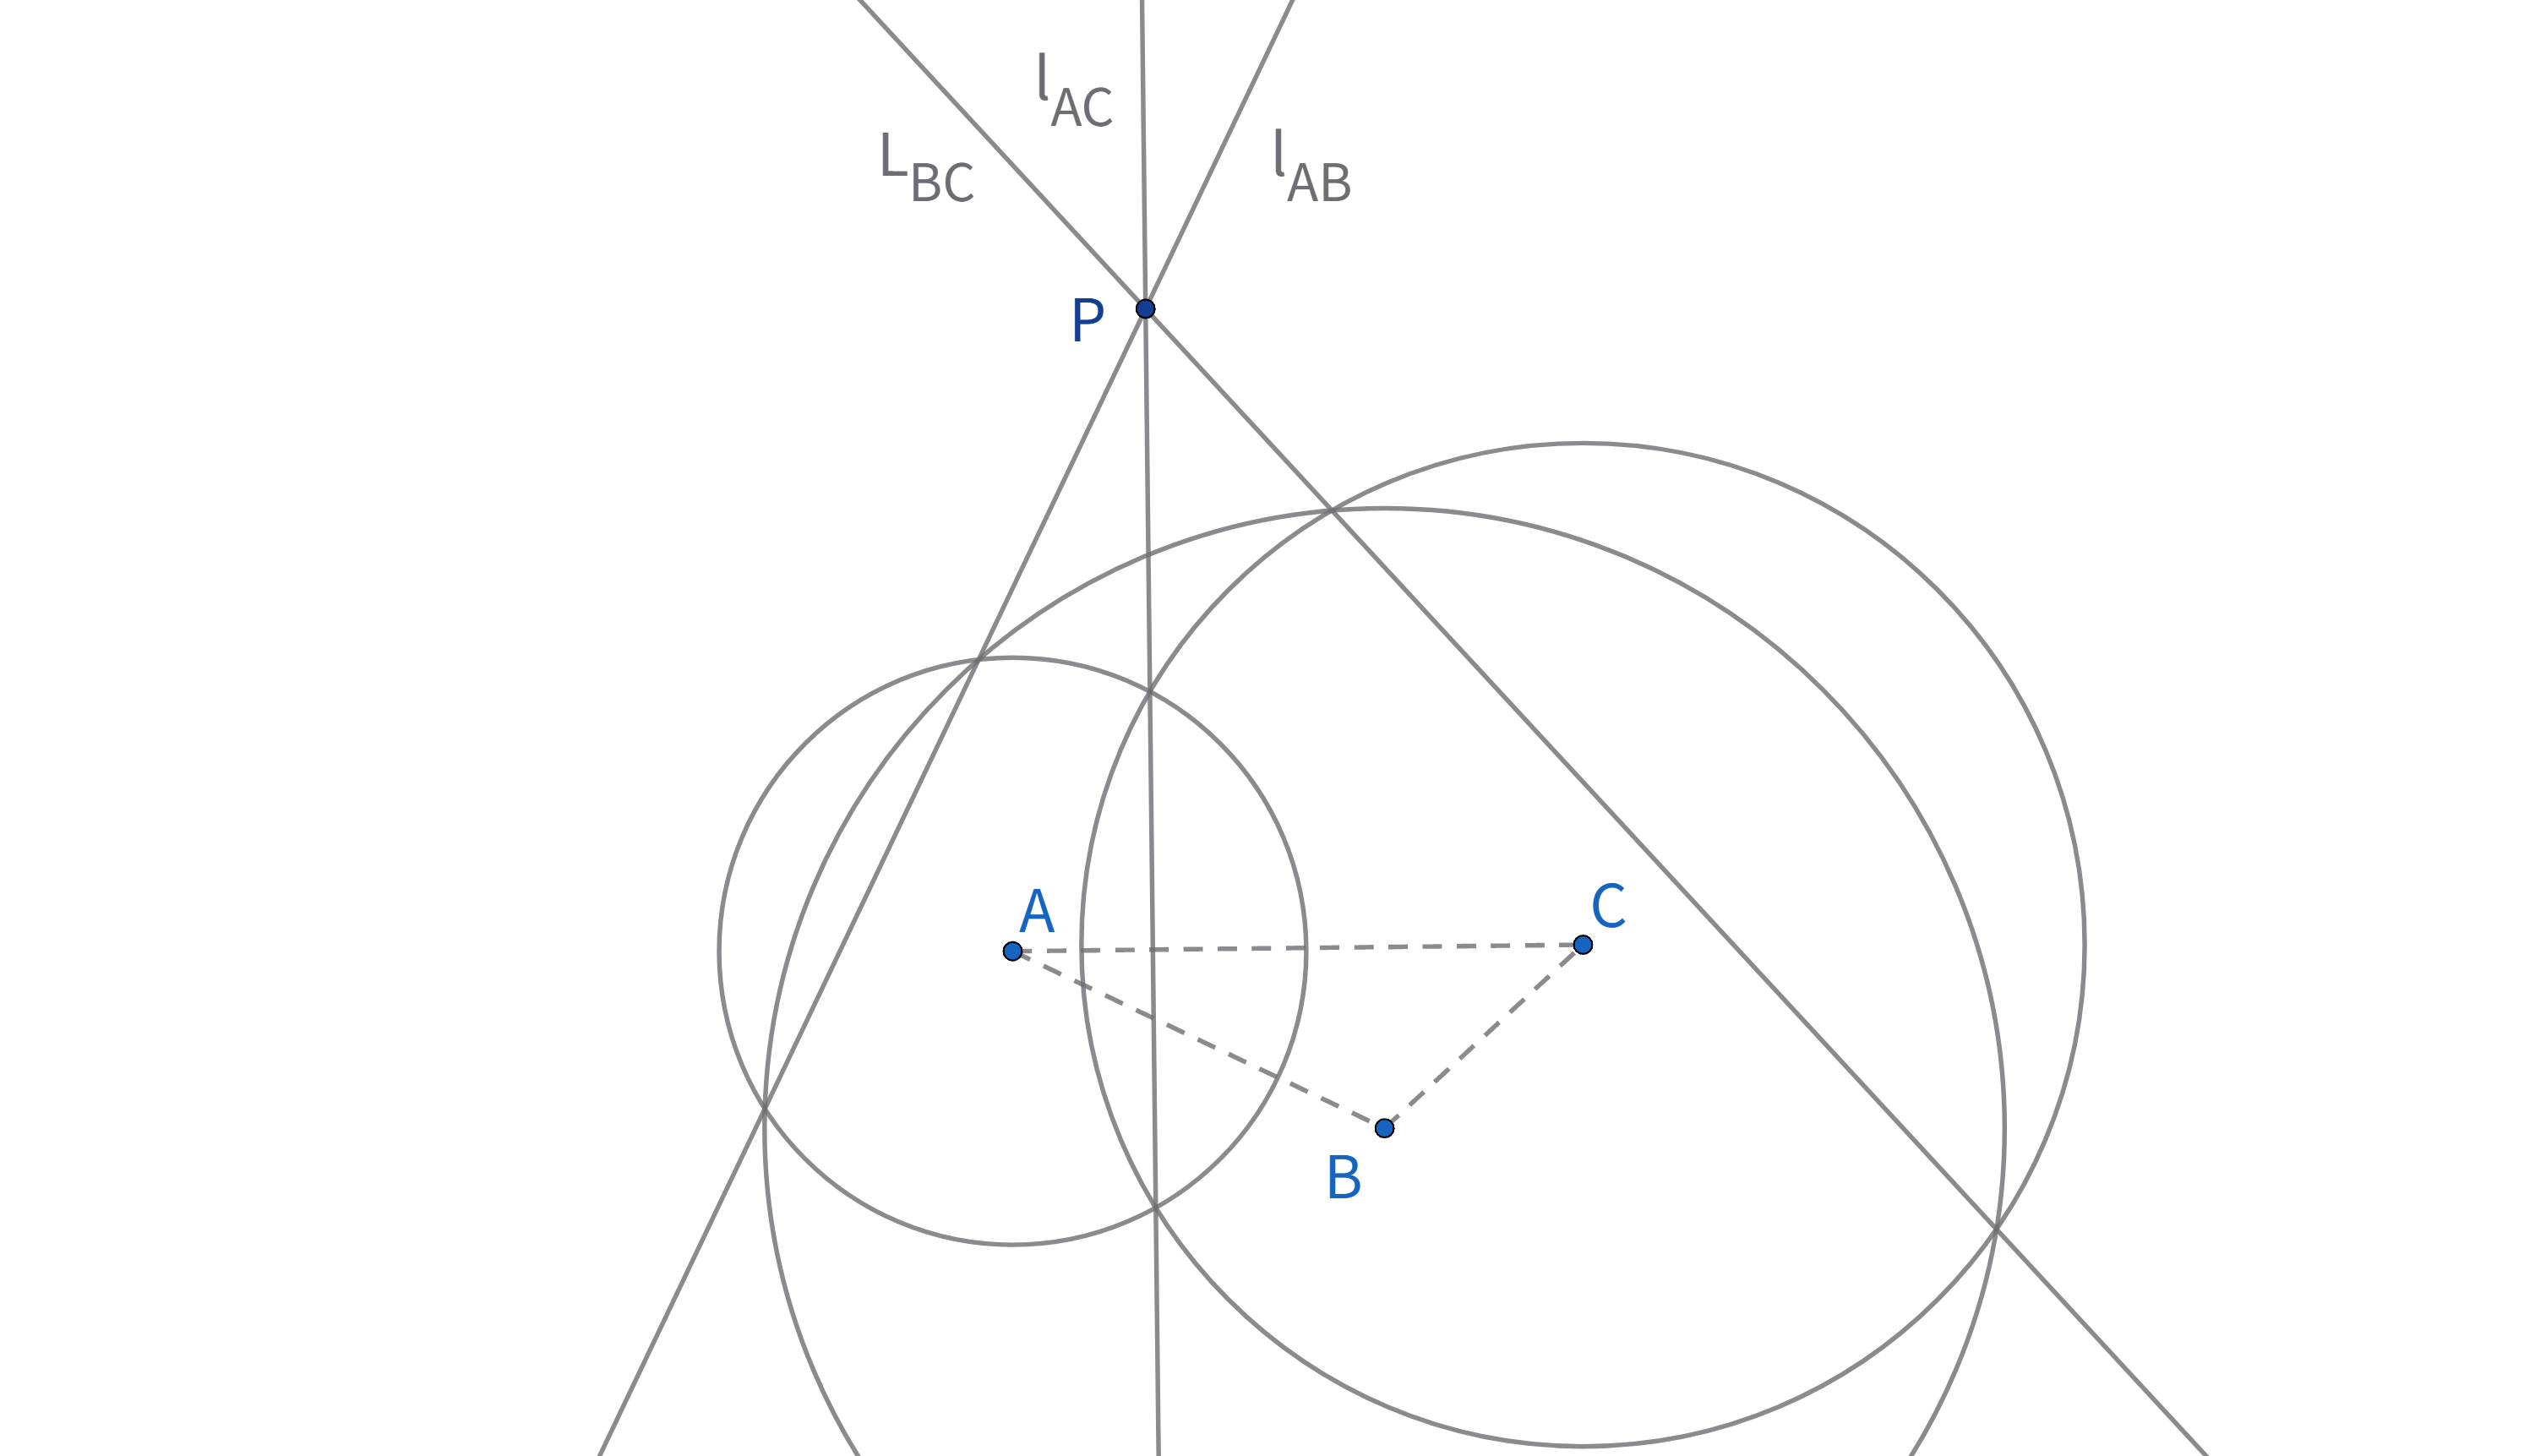
\includegraphics[width=0.8\linewidth]{figures/根心.png}
    \caption{根心}
\end{figure}